\documentclass[11pt]{article}

\usepackage{float}
\usepackage{multicol}
\usepackage{graphicx}
\usepackage{hyperref}
\hypersetup
{
    colorlinks=true,
    linkcolor=black,
    filecolor=blue,      
	urlcolor=blue,
	citecolor=black
}

\title{Machine Learning -- Homework 2}
\author{Andrea Gasparini \\ \texttt{1813486}}
\date{December 2020}

\begin{document}

	\maketitle

	\tableofcontents	

	\newpage


	\section{Introduction}
	The goal of this Homework was to solve an image classification problem with
	objects typically available in a home environment.

	\begin{multicols}{2}
		\begin{itemize}
			\item \textit{accent plate}
			\item \textit{breadsticks}
			\item \textit{cereals box}
			\item \textit{cocoa drink bottle}
			\item \textit{nitrile gloves}
			\item \textit{paper bag}
			\item \textit{pears}
			\item \textit{plastic fork}
		\end{itemize}
	\end{multicols}	



	\section{Dataset}
	The dataset contains \textbf{8221} samples and it's based on a 8 classes subset of the
	\href{https://sites.google.com/diag.uniroma1.it/robocupathome-objects/home}{RoboCup@Home-Objects dataset}.
	For each class we have a folder containing all the related samples.

	\begin{figure}[H]
		\centering
		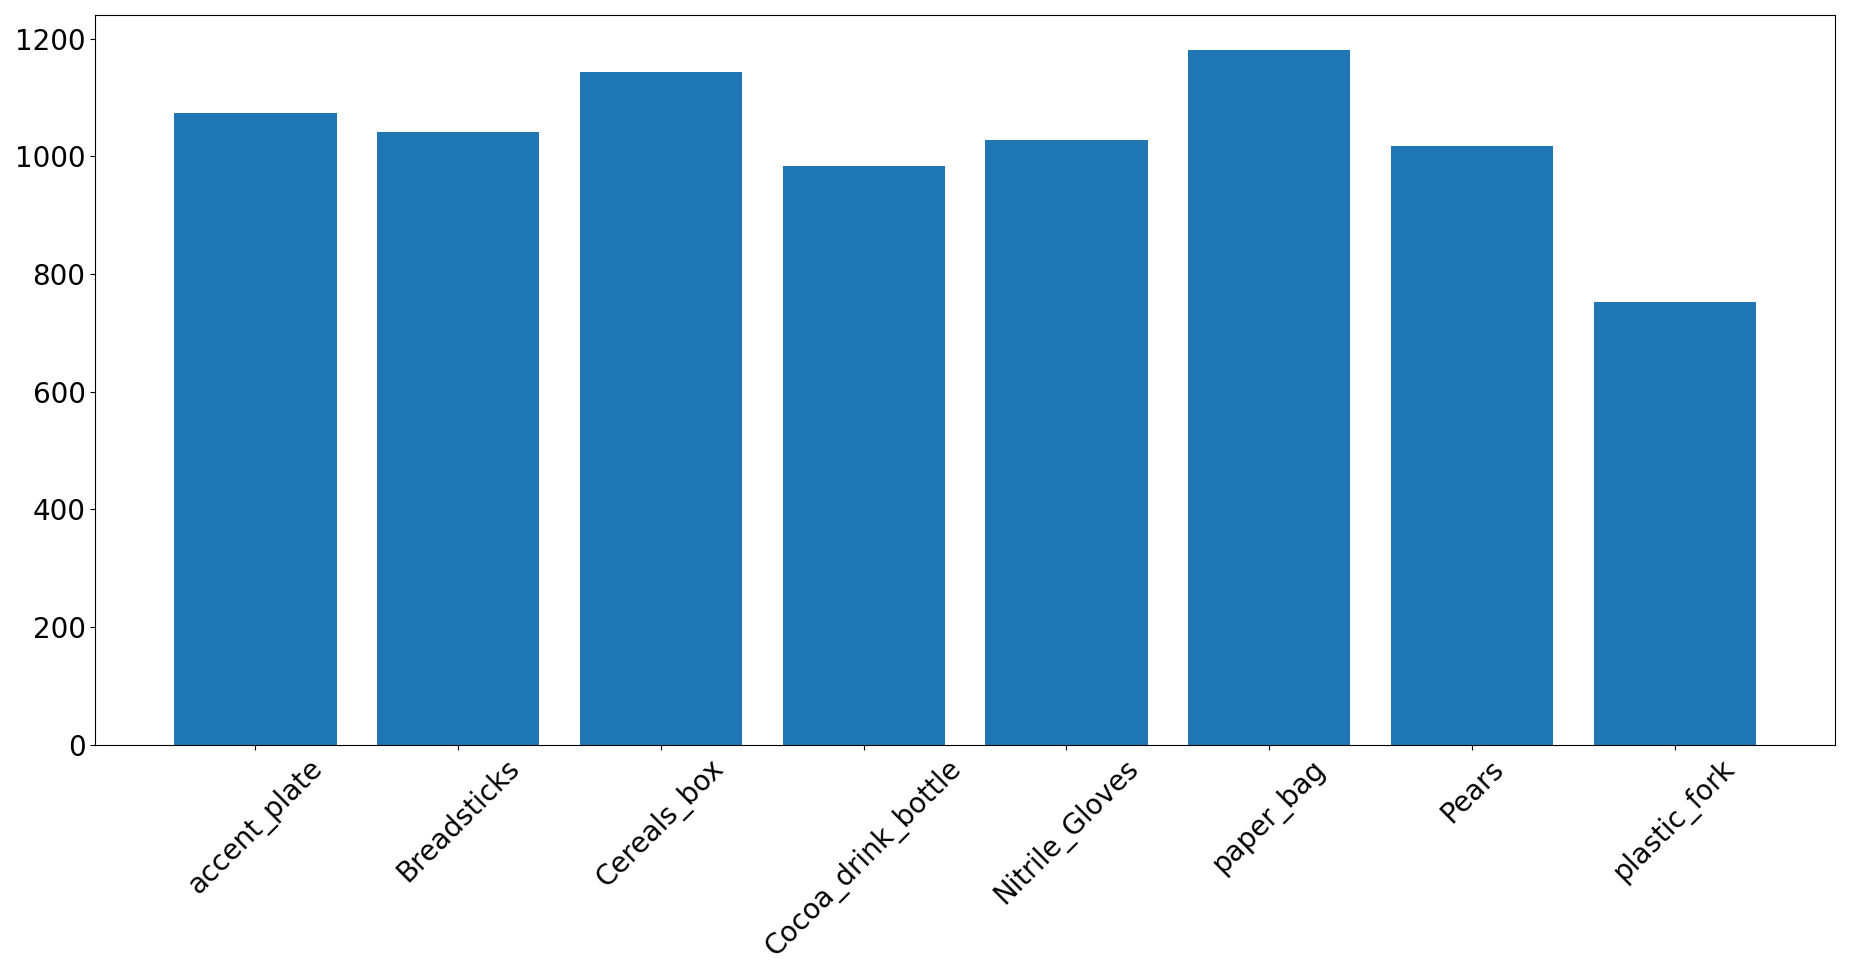
\includegraphics[width=\textwidth]{assets/dataset.png}
		\caption{Distribution of the dataset's 8 classes}
	\end{figure}


	\begin{figure}[H]
		\centering
		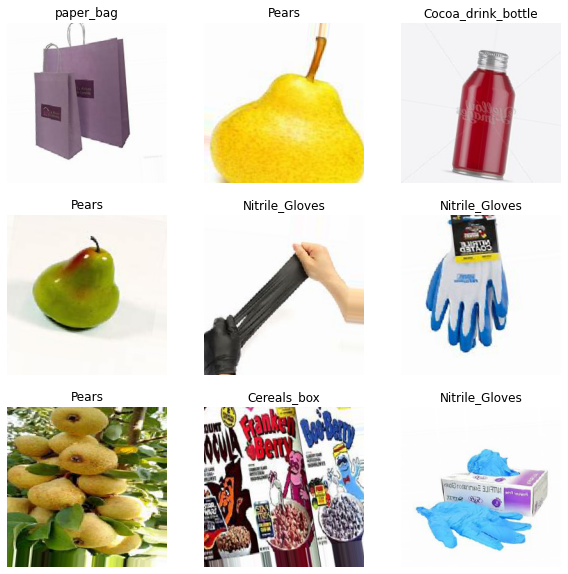
\includegraphics[width=\textwidth]{assets/dataset_samples.png}
		\caption{10 random samples from the dataset}
	\end{figure}



	\section{Preprocessing}
	The first thing I did is the dataset splitting in two subsets for training and validation,
	respectively 70\% and 30\% of the original one.


	\subsection{Data augmentation}
	Data augmentation includes techniques used to generate \textit{new} training
	samples from the original ones by applying random jitters and transformations,
	but at the same time ensuring that the class labels of the data are not changed.
	These kind of techniques are useful to reduce overfitting and they usually provide
	an increase in testing accuracy, at the expense of a slight worsening in training accuracy.
	In our case I obtained an increase in the performance by 5 to 10\% applying
	flipping, rotations and zooming.
	

\end{document}